\chapter{Introducci'on}
La programación orientada a objetos es uno paradigma de suma importancia dentro de la programación por lo que es basico conocerlo, y resulta muy útil que los estudiantes que cursan carreras técnicas o universitarias enfocadas al ámbito de la programación tengan un alto conocimiento de esto, sin embargo a pesar de llevarla como materia, les es difícil aprenderla por los amplios conceptos que maneja. Esto tambien conlleva a otro problema, que es la deserción de los alumnos de la carrera. La reprobación estudiantil es un problema añejo y complejo en las instituciones de educación superior. El propósito de este proyecto es aumentar el egreso de estudiantes.

\section{Problematica}
\subsection{Ingeniería es el área con mayor tasa de abandono escolar universitario, particularmente aquellas vinculadas con la informática}
El mercado laboral sufre el dilema vocacional porque las carreras más demandadas son las menos elegidas por los estudiantes después del primero año, ya que el abandono es mayor en el área de ingeniería y especialmente en informática. El foro profesional de los ingenieros técnicos en España advierte que el déficit de profesionales en el área de software y telecomunicaciones derivará en la importancia masiva de ingenieros dentro de una década.

\subsection{Problemas del aprendizaje de la programación orientada a objetos}
El problema del aprendizaje de la programación orientada a objetos se manifiesta toda vez que es una materia compleja que implica la integración de muchos elementos como son el paradigma orientado a objetos, el lenguaje de programación, el entorno de desarrollo, la metodología de desarrollo, el lenguaje de modelado, los patrones de desarrollo y la lógica de programación. Por lo tanto los alumnos se encuentran ante una cantidad abrumadora de conceptos en un periodo corto de tiempo, lo que dificulta su asimilaci'on y el desarrollo de las habilidades para generar l'ineas de c'odigo como lo explica \cite{spigariol2013ensenando}:

\begin{minipage}{0.9\linewidth}
	 \vspace{5pt}
	 \begin{small}
	 	``Los docentes ve'ian en los estudiantes que el uso del lenguaje representaba una curva de aprendizaje abrupta en los primeros momentos de la materia ya que requieren el manejo de una cantidad 'amplia de conceptos antes de poder realizar algo relativamente sencillo (...). La disociaci'on entre teor'ia y pr'actica que se generaba era ciertamente contraproducente y dificultaba el proceso de aprendizaje."
	 \end{small}
\end{minipage}

Debido a que los conceptos que se tratan en la asignatura de programación orientada a objetos son muchos y en algunos casos difíciles de comprender por el alto nivel de abstracción, esto se configura como un factor que dificulta el aprendizaje, esto se ha visto reflejado por ejemplo cuando los estudiantes generalmente no distinguen entre lo que es una clase y un objeto.

Además la forma de enseñar la asignatura de programación orientada a objetos es muy similar a la de la programación estructurada, primero se tratan temas básicos del lenguaje de programación, como son la declaraciones de los tipos de datos, las estructuras de control y las sentencias de condición, para posteriormente enseñar lo que son las clases, objetos y los principales temas propios del paradigma orientada a objetos, esto contribuye a que los estudiantes sientan que continúan con el mismo paradigma de programación estructurada.

En virtud de que los estudiantes no logran asimilar este cambio de paradigmas, usan el lenguaje de programación orientada a objetos como un lenguaje de programación estructurada, por consiguiente no resuelven problemas diseñando clases.

Así pues los estudiantes al llegar a la asignatura de programación orientada a objetos se enfrentan de entrada a dos problemas, la percepción que tienen de dificultad y por otro lado el proceso de transición del paradigma estructurado hacia el paradigma orientado a objetos.

\section{Objetivo general}
Desarrollar una aplicación móvil con la herramienta de Android Studio, para que las personas interesadas en la programación puedan aprender de una mejor manera el paradigma de programación orientada a objetos, y así puedan adquirir y/o reforzar su conocimiento de este paradigma. 

\section{Objetivos espec'ificos} 
\begin{itemize}
\item Proporcionar a los estudiantes y personas interesadas en la programación, información acerca del paradigma de programación orientada a objetos.
\item Evaluar el conocimiento de los usuarios de la aplicación con exámenes al finalizar un tema.
\item Diseñar una interfaz de tal forma que el usuario pueda aprender a utilizar la aplicación en el menor tiempo posible.
\item Programar la aplicación de tal forma de que no consuma muchos recursos al usarla en un celular.
\end{itemize}

\section{Justificación}
\subsection{Las TIC en la educaci'on}
De acuerdo con \cite{palaciostics} en la educaci'on el uso de las nuevas tecnolog'ias de la informaci'on ha pasado por las siguientes etapas:

\begin{figure}
	\begin{center}
		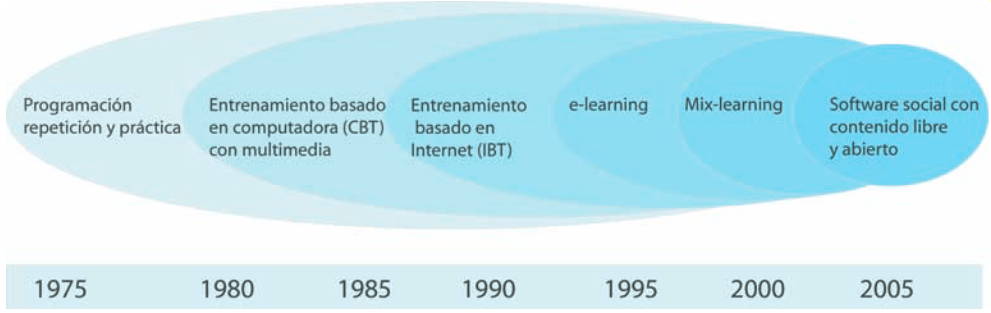
\includegraphics[scale=0.5]{img/img1.png} 
		\caption{Evoluci'on de las TIC en la educaci'on. (Basado en \cite{palaciostics})}
		\label{tic}
	\end{center}
\end{figure}

Esta evoluci'on muestra como cada vez el aprendizaje va utilizando m'as tecnolog'ia; pasando de ser 'esta simplemente una herramienta de apoyo, hasta ser la plataforma a trav'es de la cual se presentan los contenidos y eval'uan los conocimientos. 

Mix-Learning. La etapa posterior al e-learning es la aplicaci'on de una mezcla de sus herramientas con sistemas educativos tradicionales. La finalidad es dirigir m'as espec'ificamente los contenidos a los estudiantes. Es as'i que el Blend Learning, Mix Learning o Hybrid Learning se presenta como ``la combinaci'on efectiva de los diferentes modelos de reparto, modelos de ense'nanza y modelos de aprendizaje" \citep{olivares2016tic}.

\subsection{M-Learning en la educaci'on}
Seg'un la Organizaci'on de las Naciones Unidas para la Educaci'on la Ciencia y la Cultura \citep{dykes2012mobile} existen 5.9 billones de suscripciones de tel'efonos m'oviles en el mundo, contra los 7.04 billones de habitantes. Adem'as, en el a'no 2020 los dispositivos m'oviles ser'an la principal herramienta de conexi'on a internet para la mayor'ia de la poblaci'on; en Jap'on, actualmente el 75\% de su poblaci'on tiene un dispositivo m'ovil como primer medio de acceso a internet \citep{camacho2011m}. 

Asimismo, en a'nos recientes el uso de la tecnolog'ia m'ovil para fines educativos, conocido como m-learning, ha tenido un gr'an desarrollo en la educaci'on superior, ya que existen universidades de Europa y Am'erica que cuentan con sistemas de educaci'on m'ovil \citep{traxler2007defining}.

\subsection{La importancia de la programaci'on orientada a objetos}
La programaci'on Orientada a Objetos surge como el paradigma que permite manejar ampliamente las nuevas plataformas que garanticen desarrollar aplicaciones robustas, portables y reutilizables que puedan ofrecer una soluci'on a largo plazo en un mundo donde los cambios se dan a cada momento.

El desarrollo de programas orientados a objetos es un enfoque diferente del mundo inform'atico. Implica la creaci'on de modelos del mundo real y la construcci'on de programas inform'aticos basados en esos modelos.

La importancia de esta programaci'on radica en que, favorece la creaci'on de programas de calidad, fuerza en mantenimiento, en extensi'on y reutilizaci'on de programas. Est'a basada en el modo de pensar del hombre y en el modo de trabajar de la m'aquina.

Es muy importante que los estudiantes sean capaces, no s'olo de manejar los conceptos de orientaci'on a objetos, sino tambi'en de aplicarlos de manera efectiva en el desarrollo de programas.